% To add an image or include a .tex file you need to add
% \CWD
% to the relative (to the main document) path.
%
% Example:
% \begin{figure}
%   \centering
%   \includegraphics{\CWD/images/example.pdf}
% \end{figure}

Benedita é uma jovem muito criativa e interessada em ciência. Desde criança, ela aprendeu que o conhecimento racional que a humanidade adquiriu ao longo da história permitiu com que a qualidade de vida melhorasse. Desde aquela época, ela já sabia que fazia uma enorme diferença ações simples, como tomar banho diariamente, escovar os dentes após as refeições, lavar as mãos após usar o banheiro e consumir alimentos assepsiados. Entretanto, o que a maravilhou mais desde sempre foi a vacina, um resultado da sapiência que tornou possível a imunização contra doenças contagiosas.

A jovem aprendeu, logo no ensino fundamental, que o primeiro indício de vacina surgiu na China, durante o século X. Na época a população sofria com uma doença febril viral denominada varíola, produtora pústulas que deixavam cicatrizes, e não tinha cura. O método usado para a imunização era bem peculiar, pois os pesquisadores da época transformavam cascas de feridas da varíola em um pó contendo o vírus inativado e, posteriormente, espalhavam nas chagas das pessoas contaminadas. Esse método ficou conhecido como variolação.

Após alguns séculos, especificamente em 1796 na Inglaterra, Edward Jenner criou uma técnica de criação de vacinas que são semelhantes às atuais. Ao perceber que moradores de áreas rurais que haviam contraído \textit{cowpox}, a varíola bovina, não ficavam doentes com a versão humana da doença. Jenner fez um experimento e aplicou no menino James Phipps de oito anos, uma pequena dose desta varíola bovina. O garoto ficou doente, porém manifestou uma forma branda da enfermidade. Após sua recuperação, Jenner introduziu na criança o vírus da doença humana em sua forma mais fatal, retirado de uma ordenhadeira. O menino, já imune, não desenvolveu a varíola. A vacina, palavra que vem de ``\textit{vacca}'' justamente pelo contexto histórico, tornou possível a erradicação da varíola e de muitas outras doenças mortais que acometem a humanidade.

\begin{figure}[!htb]
	\centering
	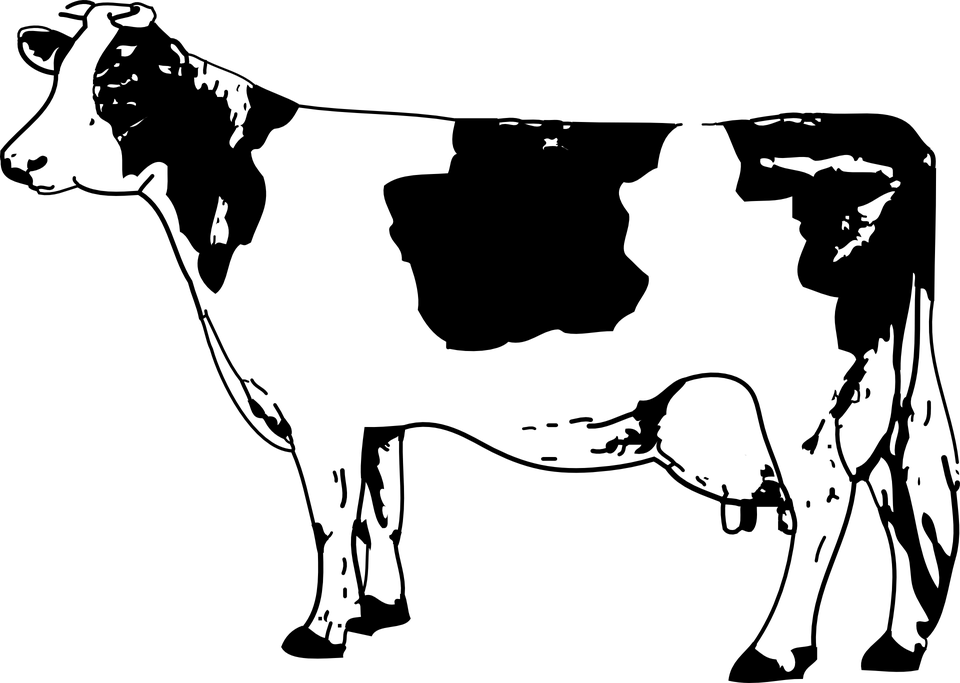
\includegraphics[width=0.5\textwidth]{\CWD/vaca.png}
\end{figure}

Desde então, o conhecimento humano se desenvolveu através de estudos sérios e éticos. Há hoje diferentes tecnologias empregadas, que vão desde as clássicas -- como as vacinas de vírus inteiros inativados, subunitárias proteicas, recombinantes e VLP -- às novas plataformas de ácidos nucleicos (DNA e mRNA) e de vetores virais.

Para Benedita, a vacina é tão vital, fascinante, racional e útil, que ela acha muito estranho alguém negar em se vacinar. Ainda do mais, ela pensa ser um bananão aquela pessoa que prefere acreditar em \textit{fake news} do que em informações científicas.

Pensando nesse contexto e sendo uma amante do estoicismo, Benedita deseja ter ao seu redor apenas pessoas que valorizam a ciência. Ela não deseja a amizade de alguém que pode colocar em risco ela e seus respectivos amados. Para isso, ela precisa saber se a pessoa é negacionista ou não. Se for, ela simplesmente deseja, respeitosamente, a distância.

Benedita pediu aos times da Maratona Mineira para criar um programa que selecione os candidatos a amizade. Ela é uma pessoa muito legal, carinhosa, divertida e preocupada com o bem estar do próximo.

\section*{Entrada}

A entrada possui uma linha contendo um valor inteiro $V$, que vale $1$, quando o candidato a amigo é negacionista a ponto de não tomar vacinas cuja eficácia são cientificamente comprovadas, e $0$ caso contrário.

\section*{Saída}

A saída possui uma linha com um valor inteiro $A$, que vale $1$ quando o candidato é aceito por Benedita para se ter a amizade dela, de acordo com o critério que ela adota, e $0$ caso contrário.

\section*{Restrições}

\begin{itemize}
	\item $1 \leq V \leq 0$
\end{itemize}


\section*{Exemplos}

\exemplo
